\iffalse
\section{xe}
\chapter{2024}
\author{ai24btech11036}
\fi

%\begin{enumerate}

	\item If '$\to$' denotes increasing order of intensity, then the meaning of the words $\sbrak{\text{walk} \to \text{jog} \to \text{sprint}}$ is analogous to $\sbrak{\text{bothered} \to \rule{1cm}{0.2pt} \to \text{daunted}}$. Which one of the given options is appropriate to fill the blank?
		\hfill{2024-XE}
	\begin{enumerate}
	\item phased 
	\item phrased
	\item fazed
	\item fused
	\end{enumerate}

\item Two wizards try to create a spell using all the four elements, \textit{water, air, fire, and earth}. For this, they decide to mix all these elements in all possible orders. They also decide to work independently. After trying all possible combination of elements, they conclude that the spell does not work. \\
How many attempts does each wizard make before coming to this conclusion,
independently?

\hfill{2024-XE}


	\begin{enumerate}
		\item 24
		\item 48
		\item 16
		\item 12
	\end{enumerate}

\item In an engineering college of 10,000 students, 1,500 like neither their core branches nor other branches. The number of students who like their core branches is 1/4 th of the number of students who like other branches. The number of students who like both their core and other branches is 500. \\
The number of students who like their core branches is
\hfill{2024-XE}

	\begin{enumerate}
		\item 1,800
		\item 3,500
		\item 1,600
		\item 1,500
	\end{enumerate}

\item For positive non-zero variables $x$ and $y$, if
	\begin{align*}
		\ln \brak{\frac{x+y}{2}}=\frac{1}{2} \cbrak{\ln \brak{x} + \ln \brak{y}}
	\end{align*}
then, the value of $\frac{x}{y} + \frac{y}{x}$ is
\hfill{2024-XE}

	\begin{enumerate}
		\item 1
		\item $\frac{1}{2}$
		\item 2
		\item 4
	\end{enumerate}
\item In the sequence 6, 9, 14, $x$, 30, 41, a possible value of $x$ is
\hfill{2024-XE}

	\begin{enumerate}
		\item 25
		\item 21
		\item 18
		\item 20
	\end{enumerate}

\end{enumerate}

%\section{Questions with two marks each}
%\begin{enumerate}
\item Sequence the following sentences in a coherent passage.\\
	P: This fortuitous geological event generated a colossal amount of energy and heat that resulted in the rocks rising to an average height of 4 km across the contact zone. \\
	Q: Thus, the geophysicists tend to think of the Himalayas as an active geological event rather than as a static geological feature.\\
	R: The natural process of the cooling of this massive edifice absorbed large quantities of atmospheric carbon dioxide, altering the earth's atmosphere and making it better suited for life. \\
	S: Many millennia ago, a breakaway chunk of bedrock from the Antarctic Plate collided with the massive Eurasian Plate. 
\hfill{2024-XE}

	\begin{enumerate}
		\item QSPR
		\item QPSR
		\item SPQR
		\item SRPQ
	\end{enumerate}

\item A person sold two different items at the same price. He made 10\% profit in one item, and 10\% loss in the other item. In selling these two items, the person made a total of
\hfill{2024-XE}

	\begin{enumerate}
		\item 1\% profit
		\item 2\% profit
		\item 1\% loss
		\item 2\% loss
	\end{enumerate}

\item The pie charts depict the shares of various power generation technologies in the total electricity generation of a country for the years 2007 and 2023. \\
	\begin{figure}[ht]
		\centering
		\begin{tikzpicture}

% Pie Chart for 2007
\node at (0, 0) {
    \begin{tikzpicture}
        \node at (0, 2.2) {Year 2007};
        
        \begin{scope}
            % Sectors for 2007
            \fill[blue!50] (0,0) -- (0:1.5) arc (0:126:1.5) -- cycle; % Coal 35%
            \fill[orange!50] (0,0) -- (126:1.5) arc (126:216:1.5) -- cycle; % Gas 25%
            \fill[yellow!50] (0,0) -- (216:1.5) arc (216:324:1.5) -- cycle; % Hydro 30%
            \fill[gray!50] (0,0) -- (324:1.5) arc (324:342:1.5) -- cycle; % Wind 5%
            \fill[pink!50] (0,0) -- (342:1.5) arc (342:360:1.5) -- cycle; % Solar 5%
        \end{scope}
        
        % Labels for 2007
        \node[fill=gray!30, rounded corners] at (0.8, 1.1) {Coal 35\%};
        \node[fill=gray!30, rounded corners] at (-0.8, 0.3) {Gas 25\%};
        \node[fill=gray!30, rounded corners] at (-0.5, -1) {Hydro 30\%};
        \node[fill=gray!30, rounded corners] at (0.8, -0.5) {Wind 5\%};
        \node[fill=gray!30, rounded corners] at (1.2, 0.2) {Solar 5\%};
    \end{tikzpicture}
};

% Pie Chart for 2023
\node at (5, 0) {
    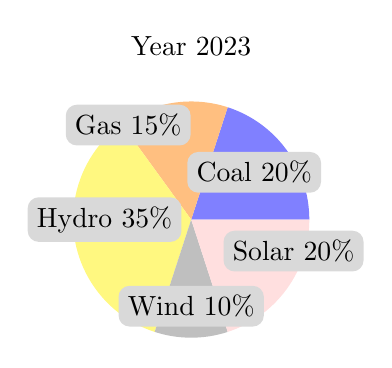
\begin{tikzpicture}
        \node at (0, 2.2) {Year 2023};
        
        \begin{scope}
            % Sectors for 2023
            \fill[blue!50] (0,0) -- (0:1.5) arc (0:72:1.5) -- cycle; % Coal 20%
            \fill[orange!50] (0,0) -- (72:1.5) arc (72:126:1.5) -- cycle; % Gas 15%
            \fill[yellow!50] (0,0) -- (126:1.5) arc (126:252:1.5) -- cycle; % Hydro 35%
            \fill[gray!50] (0,0) -- (252:1.5) arc (252:288:1.5) -- cycle; % Wind 10%
            \fill[pink!50] (0,0) -- (288:1.5) arc (288:360:1.5) -- cycle; % Solar 20%
        \end{scope}
        
        % Labels for 2023
        \node[fill=gray!30, rounded corners] at (0.8, 0.6) {Coal 20\%};
        \node[fill=gray!30, rounded corners] at (-0.8, 1.2) {Gas 15\%};
        \node[fill=gray!30, rounded corners] at (-1.1, 0) {Hydro 35\%};
        \node[fill=gray!30, rounded corners] at (0, -1.1) {Wind 10\%};
        \node[fill=gray!30, rounded corners] at (1.3, -0.4) {Solar 20\%};
    \end{tikzpicture}
};

\end{tikzpicture}

	\end{figure}
	%insert pie chart
The renewable sources of electricity generation consist of Hydro, Solar and Wind. Assuming that the total electricity generated remains the same from 2007 to 2023, what is the percentage increase in the share of the renewable sources of electricity generation over this period?
\hfill{2024-XE}

	\begin{enumerate}
		\item 25\%
		\item 50\%
		\item 77.5\%
		\item 62.5\%
	\end{enumerate}

\item A cube is to be cut into 8 pieces of equal size and shape. Here, each cut should be straight and it should not stop till it reaches the other end of the cube. \\
The minimum number of such cuts required is
\hfill{2024-XE}

		\begin{enumerate}
			\item 3
			\item 4
			\item 7
			\item 8
		\end{enumerate}

\item In the $4 \times 4$ array shown below, each cell of the first three rows has either a cross $\brak{ \times}$ or a number \\
	%insert table here
	\begin{table}[ht]
		\centering
		   \begin{tabular}{llll}
            &Group I & &Group II \\
            P. &Regain of strength with time & 1. &Boiling \\
            Q.& Loss of strength due to cyclic loading & 2. &Liquefaction \\
            R. &Loss of strength due to upward seepage & 3.& Thixotropy \\
            S. &Loss of strength due to remolding & 4. &Sensitivity \\
        \end{tabular}
	\end{table}
The number in a cell represents the count of the immediate neighboring cells (left, right, top, bottom, diagonals) NOT having a cross $\brak{ \times}$. Given that the last row has no crosses $\brak{ \times}$, the sum of the four numbers to be filled in the last row is
\hfill{2024-XE}

		\begin{enumerate}
			\item 11
			\item 10
			\item 12
			\item 9
		\end{enumerate}

%\end{enumerate}

%\section{XE-A Questions with one mark each}

%\begin{enumerate}

\item Let 
	\begin{align*}
		f\brak{x}= \begin{cases}
			 	\pi + x, & -\pi \leq x < 0, \\
				0, & 0 \leq x < \pi,
		\end{cases}
	\end{align*}
with $f\brak{x + 2\pi}=f\brak{x}$. If $F\brak{x}$ represents the fourier series of $f\brak{x}$, then the value of $F\brak{-\frac{\pi}{2}}+F\brak{0}$ is
\hfill{2024-XE}

		\begin{enumerate}
			\item 0
			\item $\frac{\pi}{2}$
			\item $\pi$
			\item $\frac{3\pi}{2}$
		\end{enumerate}

\item Let $y$ be a non-zero quadratic polynomial satisfying the differential equation 
	\begin{align*}
		\brak{2+x^2}\frac{d^2y}{dx^2}+x\frac{dy}{dx}-ky=0,
	\end{align*}
		where $k$ is a real constant. If $y\brak{1}=1$, then the value of the integral
		\begin{align*}
			\int_0 ^1 2y dx
		\end{align*}
		is
\hfill{2024-XE}

		\begin{enumerate}
			\item $\frac{1}{3}$
			\item $\frac{2}{3}$
			\item 1
			\item $\frac{4}{3}$
		\end{enumerate}

\item There are four cities namely, $C_1$, $C_2$, $C_3$ and $C_4$. The cities are directly connected by four roads as shown in the picture given below, that is, $C_1$ is connected with $C_2$, $C_2$ is coonected with $C_3$, $C_3$ is connected with $C_4$, and $C_4$ is connected with $C_1$. The probability of getting any road independently is $\frac{1}{3}$. Let $E_1$ be the event of travelling from $C_1$ to $C_3$ via $C_2$ and $E_2$ be the event of traveling from $C_1$ to $C_3$ via $C_4$. The, which of the following statements is correct?
	\begin{figure}[ht]
		\centering
		\begin{tikzpicture}
    % Draw rectangle
    \draw[thick] (0, 0) rectangle (4, 2);
    
    % Label vertices
    \node[below left] at (0, 0) {$C_1$};
    \node[below right] at (4, 0) {$C_2$};
    \node[above right] at (4, 2) {$C_3$};
    \node[above left] at (0, 2) {$C_4$};
\end{tikzpicture}


	\end{figure}
\hfill{2024-XE}

		%insert diagram
		\begin{enumerate}
			\item $P\brak{E_1 \cup E_2} = \frac{56}{81}$
			\item $P\brak{E_1 \cup E_2}= \frac{8}{9}$
			\item $P\brak{E_1 \vert E_2} \neq P\brak{E_1}=\frac{4}{9}$
			\item $P\brak{E_1 \cap E_2} = 0$
		\end{enumerate}
\newpage
	\item Assume that $f:\cbrak{0,1} \to \mathbb{R}$ is continuous on $\sbrak{0,1}$ and differentiable on $\brak{0,1}$ such that $f\brak{x+h}=f\brak{x}+hf\prime \brak{x+\theta h}$ for some $0< \theta <1$. If $f\brak{x}=x^2\brak{1+x}$, and $\theta$ is expressed in terms of $x$ and $h$, then the value of 
		$$ \lim _{h \to 0} \theta \brak{x,h}$$ is
\hfill{2024-XE}

		\begin{enumerate}
			\item $\frac{1}{3}$
			\item $\frac{1}{2}$
			\item $\frac{1}{4}$
			\item $\frac{4}{5}$
		\end{enumerate}

\item Let $A$ be a $3 \times 3$ matrix whose eigenvalues are 2, 3, 4 and let $I$ be the identity matrix of order 3. If
	$$ A^{-1}=\frac{1}{2k} \brak{A^2 -A} + \frac{13}{k} I$$
		for some integer $k \neq 0$, then the value of $k$ is \rule{1cm}{0.2pt}
\hfill{2024-XE}


\item For some integer $k$, the differential equation 
		$$ x^2 \frac{d^2 y}{dx^2} -3x\frac{dy}{dx}+\brak{k+2}y-0$$
	is transformed into $\brak{D-2}^2 y=0$, where $D=\frac{d}{dt}$ and $t=\log _e x$. Then, the value of $k$ is \rule{1cm}{0.2pt}

 \hfill{2024-XE}


\item The approximate value (\textit{rounded off to two decimal places}) of the integral 
	$$ \int ^{1/2} _{0} e^{-x^2} dx,$$
	using the Trapezoidal rule with step-size $h=\frac{1}{8}$, is \rule{1cm}{0.2pt}
\hfill{2024-XE}


%\end{enumerate}

%\section{Questions with two marks each}

%\begin{enumerate}

	\item Consider $f\brak{z}=e^z$, where $z=x+iy$ and $i=\sqrt{-1}$. Which of the following statemnets is correct?

	 \hfill{2024-XE}

		\begin{enumerate}
			\item $f$ is periodic
			\item $f$ is not periodic
			\item $\abs{f}=1$
			\item $\text{arg}\brak{f}=y \pm n \pi$ for all $n=0,1,2 \ldots$
		\end{enumerate}

	\item Let $P$ and $Q$be two square matrices of the same order. Then, which of the following matrices is/are necessarily equal tp $\brak{P+2Q}^2$?
	\hfill{2024-XE}

		\begin{enumerate}
			\item $P^2 +4PQ +4Q^2$
			\item $P\brak{P+2Q}+Q\brak{2P+Q}$
			\item $\brak{P+2Q} \brak{2Q+P}$
			\item $P^2 +2PQ+2QP+4Q^2$
		\end{enumerate}

	\item If 
		$$ \int _0 ^{\alpha} \int_{\sqrt{x/{\alpha}}} ^1 e^{y^3}dydx=e-1, \, \alpha>0,$$
		then the value (\textit{in integer}) of $\alpha$ is \rule{1cm}{0.2pt}
	\hfill{2024-XE}

	
	\item Consider the vector field $\vec{F}=\brak{2x+y^2}\hat{i} + \brak{2xy+3y}\hat{j}$ and $\alpha_m =\int _{C_m} \vec{F} \cdot \vec{dr}$, $m=1,2,$ where $C_1$ is an arc of the unit circle connecting the points $\brak{1,0}$ and $\brak{0,1}$ and $C_2$ is the straight line connecting the points $\brak{1,0}$ and $\brak{0,1}$. The the value (\textit{in integer}) of $2\brak{\alpha_1 ^2 +3\alpha_2 ^2}$ is \rule{1cm}{0.2pt}
	\hfill{2024-XE}


%\end{enumerate}

%\section{XE-B Questions with one mark each}

%\begin{enumerate}
	\item Which one of the following figures shows the CORRECT dependence of apparent viscosity ($\eta$) on the rate of shear strain($du/dy$) for pseudoplastic fluids?
	\hfill{2024-XE}

		\begin{enumerate}
			\item %fig1
				\begin{figure}[ht]
					\input{figs/op1.tex}
				\end{figure}
			\item %fig2
				\begin{figure}[ht]
					\input{figs/op2.tex}
				\end{figure}

			\item %fig3
				\begin{figure}[ht]
					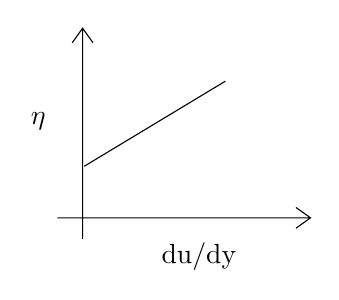
\begin{tikzpicture}[x=0.75pt,y=0.75pt,yscale=-1,xscale=1]
%uncomment if require: \path (0,235); %set diagram left start at 0, and has height of 235

%Shape: Axis 2D [id:dp7911641930796629] 
\draw  (50,169.35) -- (172,169.35)(62.2,78) -- (62.2,179.5) (165,164.35) -- (172,169.35) -- (165,174.35) (57.2,85) -- (62.2,78) -- (67.2,85)  ;
%Straight Lines [id:da49618091542370746] 
\draw    (63,144.5) -- (131,103.5) ;

% Text Node
\draw (99,180) node [anchor=north west][inner sep=0.75pt]   [align=left] {du/dy};
% Text Node
\draw (36,117.4) node [anchor=north west][inner sep=0.75pt]    {$\eta $};


\end{tikzpicture}


				\end{figure}

			\item %fig4
				\begin{figure}[ht]
					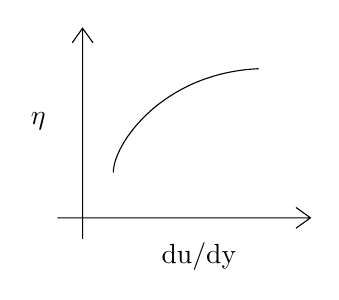
\begin{tikzpicture}[x=0.75pt,y=0.75pt,yscale=-1,xscale=1]
%uncomment if require: \path (0,235); %set diagram left start at 0, and has height of 235

%Shape: Axis 2D [id:dp7911641930796629] 
\draw  (50,169.35) -- (172,169.35)(62.2,78) -- (62.2,179.5) (165,164.35) -- (172,169.35) -- (165,174.35) (57.2,85) -- (62.2,78) -- (67.2,85)  ;
%Curve Lines [id:da20318546037237173] 
\draw    (77,147.5) .. controls (77,133.5) and (101,99.5) .. (147,97.5) ;

% Text Node
\draw (99,180) node [anchor=north west][inner sep=0.75pt]   [align=left] {du/dy};
% Text Node
\draw (122,125.4) node [anchor=north west][inner sep=0.75pt]    {$ $};
\draw (36,117.4) node [anchor=north west][inner sep=0.75pt]    {$\eta $};


\end{tikzpicture}


				\end{figure}

		\end{enumerate}

	\item The locus of temporary locations of all particles that have passed through a fixed point in the flow field at a particular instant is known as 
	\hfill{2024-XE}

		\begin{enumerate}
			\item streamline.
			\item streakline.
			\item pathline.
			\item timeline.
		\end{enumerate}
		
	\item Consider the velocities $u,v,$ and $w$ in $x-$, $y-$ and $z-$directions, respectively. The vortocity expression in the $y-z$ plane is
	\hfill{2024-XE}

		\begin{enumerate}
			\item $\frac{\partial v}{\partial x}-\frac{\partial u}{\partial y}$
			\item $\frac{\partial v}{\partial y}-\frac{\partial w}{\partial z}$
			\item $\frac{\partial w}{\partial y}-\frac{\partial v}{\partial z}$
			\item $\frac{\partial u}{\partial z}-\frac{\partial w}{\partial x}$
		\end{enumerate}

	\item For the laminar, incompressible flow over a flat plate with uniform free stream velocity, the axial pressure gradient within the boundary layer is
	\hfill{2024-XE}

		\begin{enumerate}
			\item greater than zero.
			\item less than zero.
			\item equal to zero.
			\item equal to the axial velocity gradient.
		\end{enumerate}

	\item Let $\vec{r}, \vec{V}$ and $m$ be position vector, velocity vector, and mass, respectively in a control mass system. Which one of the following properties is considered as conserved extensive property in Reynolds Transport Theorem to obtain the angular momentum equation?
	\hfill{2024-XE}

		\begin{enumerate}
			\item $\vec{r} \times m\vec{V}$
			\item $\vec{r} \times \vec{V}$
			\item $m\vec{V}$
			\item $m$
		\end{enumerate}

%\end{enumerate}
%\end{document}




				




	



	



